\begin{center}
	
	\begin{tabular}{rp{16cm}lp{20cm}}%{rl}
		
		% after \\: \hline or \cline{col1-col2} \cline{col3-col4} ...
		
		论文地址:& \href{https://dl.acm.org/doi/pdf/10.1145/3404835.3462827}{https://dl.acm.org/doi/pdf/10.1145/3404835.3462827} \\
		来源:& SIGIR, 2021 \\
		作者:& Ting Long, et al. \\
		单位:& Shanghai Jiao Tong University$_{\times 5}$ \\
		源码:& \href{https://github.com/githubg0/iekt}{iekt} \\
		
		%  slides:& \href{http://yunshengb.com/wp-content/uploads/2017/03/nips_2018_r2l_workshop_talk.pdf}{{\footnotesize Convolutional Set Matching for Graph Similarity}}\\
		
		关键词:& \textbf{Knowledge Tracing, Student assess·ment, Transformer} \\
		
		写于:& \date{2021-09-23}
		
	\end{tabular}
	
\end{center}

该论文\cite{long2021tracing}提出了一种考虑学生认知水平和获取水平时的Knowledge Tracing方法 --- Individual Estimation Knowledge Tracing(IEKT)。

\paragraph{问题定义}
以往的Knowledge Tracing方法中,默认学生的认知水平(cognition level)是不变的,且不同的学生对同样的问题给出相同的作答后,学生的只是增长是一样的。然而实际情况:不同的学生由于不同的知识水平,完成相同的练习后知识的增长是不一样的。为什么以往的方法会有以上问题呢?1)没有显示地建模学生的认知水平/能力;2)没有显示地建模学生在不同地认知和知识水平下通过练习所能获得的知识。

形式化定义:
学生的练习记录:$\mathcal{X}_{t-1} = \{(q_1, r_1), ..., (q_{t-1}, r_{t-1})\}$,$(q_t, r_t)$表示学生在$t$时做的练习及学生的回答,且$r_t \in \{0, 1\}$。
\begin{table}[h]
	\centering
	\caption{符号说明}
	\label{tab:annotation}
	\begin{tabular}{ll}
		\hline Notations & Descriptions \\
		\hline$\mathcal{X}_{t-1}$ & Student's question-answering history. \\
		$q_{i}, c_{j}$ & The question and the concept. \\
		$Q, C$ & The set of questions and the set of concepts. \\
		$\mathbf{e}_{i}^{q}, \mathbf{e}_{j}^{c}$ & The embedding of question and concept. \\
		$\hat{r}_{t}, r_{t}$ & The predicted probability and the true label. \\
		$\mathbf{M}, \mathbf{m}_{t}$ & The cognition matrix and the cognition vector. \\
		$\mathbf{S}, \mathrm{s}_{t}$ & The acquisition matrix and the accquistion vector. \\
		$\mathbf{h}_{t}$ & The knowledge state. \\
		\hline
	\end{tabular}
\end{table}
论文中相关符号说明如Tab.\ref{tab:annotation}所示。其中,每个问题$q_i$可以与多个知识点相关,每个问题$q_i$和知识点$c_i$都有对应的embedding $\boldsymbol{e}_i^q, \boldsymbol{e}_i^c$(这两者的embedding是提前准备好的),每个学生在时刻$t$的知识状态为$\boldsymbol{h}_t$。

IEKT的目标:$P(r_t | q_t, \mathcal{X}_{t-1})$。

\paragraph{IEKT}
IEKT的模型是基于GRU的,可以分为两个阶段:read和write。read的任务是预测学生的回答$\hat{r}_t$,write的任务是更新学生的知识状态$\boldsymbol{h}_t$,模型结构如Fig.\ref{fig:iekt}(b)所示。
\begin{figure}[h]
	\centering
	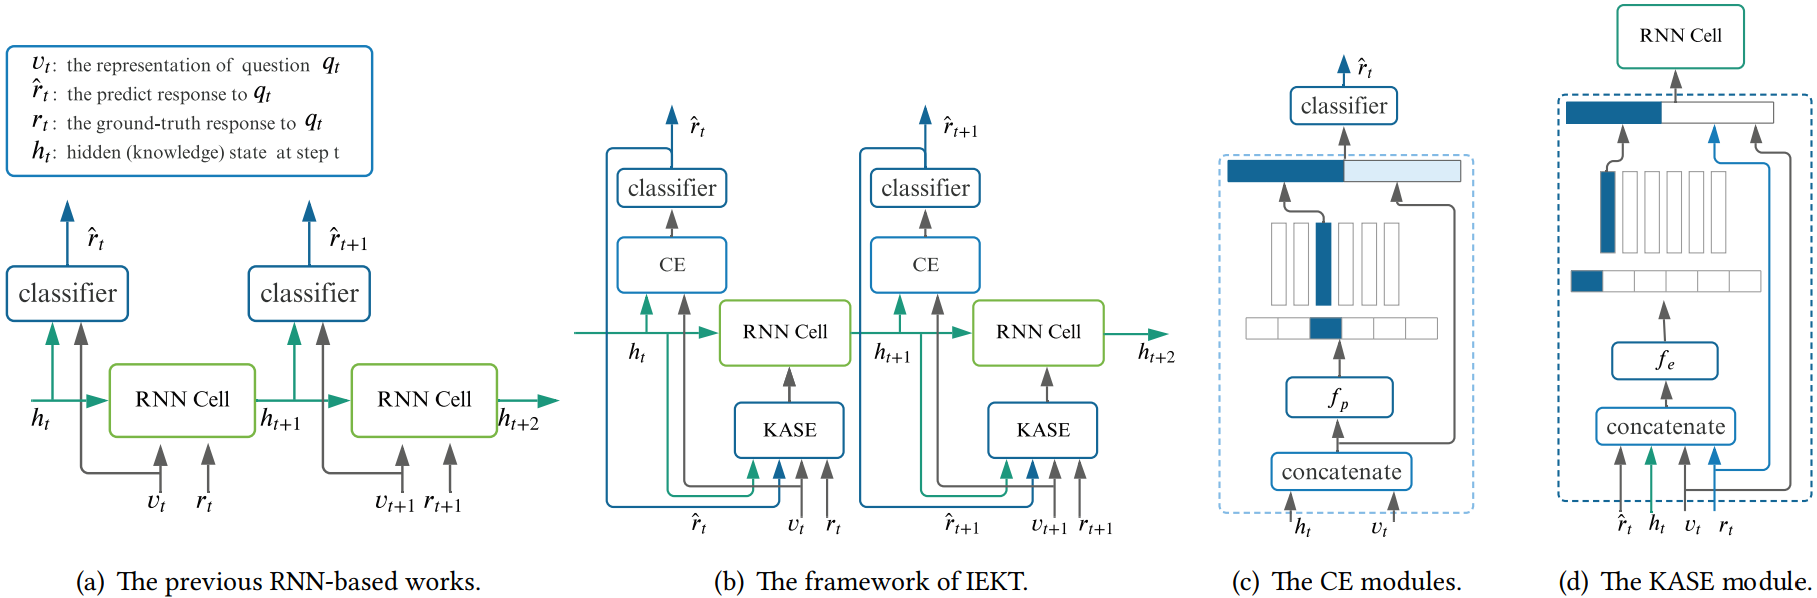
\includegraphics[width=\textwidth]{pics/iekt.png}
	\caption{The frameworks and details of IEKT}
	\label{fig:iekt}
\end{figure}

整体来看,IEKT的工作流程和其他的RNN-based模型没有很大的差别,但是IEKT在read和write阶段各引入了一个模块。

\par{\textbf{read}}\ \ \ \ IEKT在这阶段引入了Cognition Estimation(CE)模块。该模块的输入是学生的知识状态$\boldsymbol{h}_t$(也就是GRU的hidden state)和问题的表征$\boldsymbol{v}_t$(不是$\boldsymbol{e}^q$,问题表征由问题embedding和知识embedding生成,具体参见论文)。CE的输出被用于预测$\hat{r}_t$。关键在于CE的内部操作。IEKT将认知水平划分为$k$个层次,每个层次用一个向量表示,$k$个层次形成一个Cognition Matrix $\boldsymbol{M}$。CE内部会基于学生的知识状态、问题embedding和知识点embedding得到学生$t$时的cognition level。cognition level对应的向量会与学生的知识状态、问题embedding和知识点embedding一起被送进分类器去预测$\hat{r}_t$。CE内部结构见Fig.\ref{fig:iekt}(c)。

\par{\textbf{write}}\ \ \ \ IEKT在此阶段引入了Knowledge acquisition sensitivity estimation(KASE)。KASE的目的是更新学生的知识状态。IEKT将学生的knowledge acquisition sensitivity划分为$b$个层次,每个层次对应一个向量,$b$个层次形成一个knowledge acquisition sensitivity matrix $\boldsymbol{S}$。KASE内部会根据(问题的表征,学生的知识状态、预测回答、真实的回答)来选择对应的知识获取水平,再将知识获取水平与问题表征、真实回答拼接后送入GRU,GRU输出的hidden state即是学生下一时刻的知识状态。由此可见,学生的知识状态是保存在GRU中的。

另外,在CE和KASE中是是通过输入获取$\boldsymbol{M}, \boldsymbol{S}$的行索引来获取相应的向量的,这样的操作是不可导的,论文中采用强化学习中的策略梯度来实现的。除了一些显而易见的参数外,还有一些参数是需要学习的:知识点和问题的embedding $\boldsymbol{e}^c, \boldsymbol{e}^q$以及$\boldsymbol{M}, \boldsymbol{S}$。

论文中使用的数据集:ASSIST09、ASSIST12、EdNet和Junyi,使用的指标是ACC和AUC。

\paragraph{总结}

\begin{itemize}
	\item 显示地建模了学生的认知水平和知识获取水平。学生在不同的知识状态和认知水平下的知识获取能力是不一样的
	\item 将学生的知识状态保存在GRU的hidden state中
	%\item 
	
\end{itemize}

